\documentclass[11pt]{article}
% Reproducible PDF: no creation or modification date and a fixed trailer ID.
\ifdefined\pdftrailerid
  \pdfinfoomitdate=1
  \pdftrailerid{}
\fi
\usepackage[T1]{fontenc}
\usepackage{lmodern}
\usepackage[margin=1in]{geometry}
\usepackage{setspace}
\usepackage{amsmath,amssymb}
\usepackage{booktabs}
\usepackage{graphicx}
\usepackage{enumitem}
\usepackage{microtype}
\usepackage{xcolor}
\usepackage{caption}
\usepackage[authoryear,round]{natbib}
\usepackage[hidelinks]{hyperref}

\captionsetup{font=small,labelfont=bf,skip=6pt}
\setlist{itemsep=2pt,topsep=4pt}
\newcommand{\todo}[1]{\textcolor{red!70!black}{[TODO: #1]}}
\newcommand{\FC}{\mathrm{FC}}
% Shared by manuscript.tex, supplementary.tex, highlights.tex and cover_letter.tex.
\newcommand{\MsTitle}{Most faithful-looking neighborhoods in 2-D maps of trial-averaged neural responses are spurious: estimates from held-out repetitions}
\newcommand{\ChecksResultsCommit}{\texttt{3e3204e}}

% generated by make_tables.py from committed results; do not edit
\newcommand{\EegFCeight}{81--86}
\newcommand{\EegLeight}{64}
\newcommand{\EegFCsixteen}{65--75}
\newcommand{\EegLsixteen}{46}
\newcommand{\EegFCthirtytwo}{48--64}
\newcommand{\EegLthirtytwo}{23}
\newcommand{\EegNFeight}{19}
\newcommand{\EegTFeight}{5--7}
\newcommand{\EegQL}{16\%, 18\% and 16\%}
\newcommand{\EegRsaFCeight}{62--72}
\newcommand{\EegRsaLeight}{55}
\newcommand{\EegRsaNFeight}{2.0}
\newcommand{\EegCells}{10}
\newcommand{\EegBias}{$-0.008$}
\newcommand{\EegKtwentyFC}{49--63}
\newcommand{\EegKtwentyL}{31}
\newcommand{\EegPcaFC}{51--64}
\newcommand{\EegPcaL}{44}
\newcommand{\MouseFCeight}{100}
\newcommand{\MouseLeight}{99.7}
\newcommand{\MouseLsixteen}{97.7}
\newcommand{\MouseNFeight}{16}
\newcommand{\MouseQL}{15\% and 16\%}
\newcommand{\MouseRsaFCeight}{100}
\newcommand{\MouseRsaLeight}{100.0}
\newcommand{\MouseRsaNFeight}{0.9}
\newcommand{\MouseCells}{12}
\newcommand{\MouseBias}{$+0.003$}
\newcommand{\MouseTFmax}{1.4}
\newcommand{\MouseUnwhitenedNF}{46}
\newcommand{\EegUnwhitenedFC}{100}
\newcommand{\RatioEeg}{0.92}
\newcommand{\RatioMouse}{0.24}
\newcommand{\RelEeg}{0.88}
\newcommand{\RelMouse}{0.73}
\newcommand{\PosMouse}{94}
\newcommand{\MouseNonPos}{42}
\newcommand{\MouseCellsMin}{145}
\newcommand{\MouseCellsMax}{359}
\newcommand{\MouseMale}{7}
\newcommand{\MouseFemale}{3}
\newcommand{\ChkBiasMin}{$-0.014$}
\newcommand{\ChkBiasMax}{$+0.004$}
\newcommand{\ChkEegRepRows}{2700}
\newcommand{\ChkEegRepDiff}{0}
\newcommand{\ChkEegNPass}{18.8}
\newcommand{\ChkEegNFC}{81--86}
\newcommand{\ChkEegNL}{64}
\newcommand{\ChkEegNU}{92}
\newcommand{\ChkEegNCatch}{0}
\newcommand{\ChkEegNYield}{2.5--3.5}
\newcommand{\ChkEegNFCNX}{81--86}
\newcommand{\ChkEegNPassNX}{18.8}
\newcommand{\ChkEegTWPass}{19.0}
\newcommand{\ChkEegTWFC}{79--85}
\newcommand{\ChkEegTWL}{64}
\newcommand{\ChkEegTWU}{91}
\newcommand{\ChkEegTWCatch}{27--28}
\newcommand{\ChkEegTWYield}{2.7--3.9}
\newcommand{\ChkEegTWFCNX}{77--84}
\newcommand{\ChkEegTWPassNX}{14.4}
\newcommand{\ChkEegSCDPass}{32.5}
\newcommand{\ChkEegSCDFC}{86--90}
\newcommand{\ChkEegSCDL}{76}
\newcommand{\ChkEegSCDU}{94}
\newcommand{\ChkEegSCDCatch}{39--40}
\newcommand{\ChkEegSCDYield}{3.5--4.9}
\newcommand{\ChkEegSCDFCNX}{77--83}
\newcommand{\ChkEegSCDPassNX}{12.3}
\newcommand{\ChkEegCVPass}{7.9}
\newcommand{\ChkEegCVFC}{73--81}
\newcommand{\ChkEegCVL}{59}
\newcommand{\ChkEegCVU}{86}
\newcommand{\ChkEegCVCatch}{72--74}
\newcommand{\ChkEegCVYield}{1.6--2.2}
\newcommand{\ChkEegCVFCNX}{69--78}
\newcommand{\ChkEegCVPassNX}{6.1}
\newcommand{\ChkEegSEEDPass}{34.6}
\newcommand{\ChkEegSEEDFC}{87--91}
\newcommand{\ChkEegSEEDL}{77}
\newcommand{\ChkEegSEEDU}{94}
\newcommand{\ChkEegSEEDCatch}{37--39}
\newcommand{\ChkEegSEEDYield}{3.3--4.6}
\newcommand{\ChkEegSEEDFCNX}{78--84}
\newcommand{\ChkEegSEEDPassNX}{12.6}
\newcommand{\ChkEegBOOTPass}{0.0}
\newcommand{\ChkEegBOOTFC}{n.e.}
\newcommand{\ChkEegBOOTL}{n.e.}
\newcommand{\ChkEegBOOTU}{n.e.}
\newcommand{\ChkEegBOOTCatch}{100}
\newcommand{\ChkEegBOOTYield}{0.0}
\newcommand{\ChkEegBOOTFCNX}{n.e.}
\newcommand{\ChkEegBOOTPassNX}{0.0}
\newcommand{\ChkEegSHPass}{1.2}
\newcommand{\ChkEegSHFC}{47--62}
\newcommand{\ChkEegSHL}{38}
\newcommand{\ChkEegSHU}{72}
\newcommand{\ChkEegSHCatch}{97--98}
\newcommand{\ChkEegSHYield}{0.4--0.6}
\newcommand{\ChkEegSHFCNX}{36--57}
\newcommand{\ChkEegSHPassNX}{0.8}
\newcommand{\ChkMouseRepRows}{1800}
\newcommand{\ChkMouseRepDiff}{0}
\newcommand{\ChkMouseNPass}{16.1}
\newcommand{\ChkMouseNFC}{100.0}
\newcommand{\ChkMouseNL}{99.7}
\newcommand{\ChkMouseNU}{100.0}
\newcommand{\ChkMouseNCatch}{0}
\newcommand{\ChkMouseNYield}{0.0}
\newcommand{\ChkMouseNFCNX}{100}
\newcommand{\ChkMouseNPassNX}{16.1}
\newcommand{\ChkMouseTWPass}{16.3}
\newcommand{\ChkMouseTWFC}{100.0}
\newcommand{\ChkMouseTWL}{99.8}
\newcommand{\ChkMouseTWU}{100.0}
\newcommand{\ChkMouseTWCatch}{20}
\newcommand{\ChkMouseTWYield}{0.0}
\newcommand{\ChkMouseTWFCNX}{100}
\newcommand{\ChkMouseTWPassNX}{12.7}
\newcommand{\ChkMouseSCDPass}{8.8}
\newcommand{\ChkMouseSCDFC}{100.0}
\newcommand{\ChkMouseSCDL}{99.7}
\newcommand{\ChkMouseSCDU}{100.0}
\newcommand{\ChkMouseSCDCatch}{68}
\newcommand{\ChkMouseSCDYield}{0.0}
\newcommand{\ChkMouseSCDFCNX}{100}
\newcommand{\ChkMouseSCDPassNX}{6.0}
\newcommand{\ChkMouseCVPass}{2.3}
\newcommand{\ChkMouseCVFC}{100.0}
\newcommand{\ChkMouseCVL}{97.9}
\newcommand{\ChkMouseCVU}{100.4}
\newcommand{\ChkMouseCVCatch}{93}
\newcommand{\ChkMouseCVYield}{0.0}
\newcommand{\ChkMouseCVFCNX}{100}
\newcommand{\ChkMouseCVPassNX}{1.1}
\newcommand{\ChkMouseSEEDPass}{27.2}
\newcommand{\ChkMouseSEEDFC}{100.0}
\newcommand{\ChkMouseSEEDL}{99.8}
\newcommand{\ChkMouseSEEDU}{100.0}
\newcommand{\ChkMouseSEEDCatch}{41}
\newcommand{\ChkMouseSEEDYield}{0.0}
\newcommand{\ChkMouseSEEDFCNX}{100}
\newcommand{\ChkMouseSEEDPassNX}{9.4}
\newcommand{\ChkMouseBOOTPass}{0.0}
\newcommand{\ChkMouseBOOTFC}{n.e.}
\newcommand{\ChkMouseBOOTL}{n.e.}
\newcommand{\ChkMouseBOOTU}{n.e.}
\newcommand{\ChkMouseBOOTCatch}{100}
\newcommand{\ChkMouseBOOTYield}{0.0}
\newcommand{\ChkMouseBOOTFCNX}{n.e.}
\newcommand{\ChkMouseBOOTPassNX}{0.0}
\newcommand{\ChkMouseSHPass}{0.0}
\newcommand{\ChkMouseSHFC}{n.e.}
\newcommand{\ChkMouseSHL}{n.e.}
\newcommand{\ChkMouseSHU}{n.e.}
\newcommand{\ChkMouseSHCatch}{100}
\newcommand{\ChkMouseSHYield}{0.0}
\newcommand{\ChkMouseSHFCNX}{n.e.}
\newcommand{\ChkMouseSHPassNX}{0.0}
\newcommand{\ChkEegSHPassNXThirtyTwo}{9.8}
\newcommand{\ChkEegSHFCNXThirtyTwo}{20--43}
\newcommand{\ChkEegSHFCThirtyTwo}{32--52}
\newcommand{\ChkEegSHPassThirtyTwo}{14.4}
\newcommand{\ChkEegBOOTPassThirtyTwo}{1.5}
\newcommand{\ChkEegBOOTUThirtyTwo}{27}
\newcommand{\ChkEegBOOTPassSixteen}{0.15}
\newcommand{\ChkMouseMinL}{97.9}
\newcommand{\ChkEegMinL}{59}
\newcommand{\ChkEegExtraSCD}{20}
\newcommand{\ChkEegExtraSEED}{22}


\begin{document}
\onehalfspacing

\begin{titlepage}
\begin{center}
{\Large\bfseries \MsTitle\par}
\vspace{1.5em}
{\large Sooyoung Jang\par}
\vspace{0.6em}
Hanbat National University, \todo{department and full postal address}, Daejeon, Republic of Korea\par
\vspace{0.6em}
Corresponding author: Sooyoung Jang, \texttt{syjang@hanbat.ac.kr}\par
\end{center}
\vfill
\noindent\textbf{Article type:} Research article\\[2pt]
\textbf{Keywords:} t-SNE; multidimensional scaling; representational similarity analysis; trial averaging; measurement noise; dimensionality reduction; reliability
\vfill
\end{titlepage}

\section*{Abstract}
\noindent\textbf{Background:} Two-dimensional maps of trial-averaged responses, made with t-SNE or
multidimensional scaling, are read neighbor by neighbor, and analysts check them against the
averaged data. Because the map is fitted to the same noisy averages, such checks share its errors.

\noindent\textbf{New method:} We define the false comfort of a check as the share of the
neighborhoods it passes that are not faithful to the noise-free responses. We estimate it from
held-out repetitions, with a simulation--extrapolation correction for the reference's own noise and
subject-bootstrap bounds, and validate the estimator in plasmode simulations.

\noindent\textbf{Results:} Pre-specified analyses used human EEG (THINGS-EEG2; 10 subjects,
200 images) and two-photon imaging of mouse V1 (Allen Brain Observatory; 10 mice, 118 images). At 8 trials, \EegFCeight\% of the neighborhoods that passed the plug-in check were not
faithful in EEG (conservative bound \EegLeight\%), and essentially all were in mouse V1 (bound
\MouseLeight\%). Maps of cross-validated distances passed fewer neighborhoods, most of them
unfaithful. The result held in \EegCells{} and \MouseCells{} of 12 pre-specified variations.

\noindent\textbf{Comparison with existing methods:} Of six common checks computed from the
analyst's own trials, per-point trustworthiness, scDEED, cross-validated distances and recurrence
across t-SNE seeds left most false comfort in both datasets. Bootstrap and split-half recurrence
passed almost no neighborhoods at 8 trials. None removed most false comfort.

\noindent\textbf{Conclusions:} Checks computed from the same trials cannot reveal where trial
averages are wrong. Local neighborhoods of such maps should be read against held-out repetitions,
which the estimator makes practical.


\section{Introduction}\label{sec:intro}

Two-dimensional maps of condition-averaged responses are a staple of systems neuroscience.
Representational similarity analysis (RSA) displays the responses to a set of stimuli with
multidimensional scaling (MDS) \citep{kriegeskorte2008,kriegeskorte2008neuron,nili2014}, from
fMRI to time-resolved MEG \citep{cichy2014}. Object spaces are shown the same way
\citep{hebart2023}, and nonlinear embeddings such as t-SNE \citep{vandermaaten2008} and UMAP are
used to display population activity \citep{cunningham2014,gardner2022}. Such maps are read
locally: two stimuli that sit together are taken to evoke similar responses, and a stimulus's
neighbors are taken to be the stimuli it is most similar to.

It is well documented that 2-D maps distort the neighborhoods of the data they are fitted to
\citep{wattenberg2016,kobak2019,chari2023,cooley2019,lause2024}. A family of quality criteria
measures how well a map preserves those neighborhoods
\citep{venna2001,kaski2003,chen2009,lee2009,venna2010}, and per-point tools flag the points
whose neighborhoods are distorted: scDEED labels each point's embedding trustworthy or dubious
against a permutation null \citep{xia2024}, EMBEDR compares each point with embeddings of
randomized data \citep{johnson2022}, and DynamicViz measures each point's stability across
bootstrap embeddings \citep{sun2023}; see also \citet{liu2025}. All of these judge a map against
the data it was made from, or against other maps of the same data.

In neuroscience those data are averages of a limited number of noisy trials. The averages
differ from the noise-free responses they estimate, and the map is fitted to the same averages
that a check would use. A check computed from the averages therefore shares its errors with the
map, which is the conditional dependence that makes a diagnostic test look accurate when it is
judged against a reference with correlated errors \citep{vacek1985}. Related problems are known.
Hyperparameters chosen for a map's fidelity to noisy data overfit the noise, and maps are better
judged against a denoised signal \citep{lin2024}. Neighbor graphs computed from shallow data
share few neighbors with graphs from deeper data \citep{ahlmann2023}. RSA addresses trial noise
with cross-validated distance estimates \citep{walther2016,guggenmos2018} and with noise ceilings
\citep{nili2014,schutt2023}, but both concern the dissimilarity matrix as a whole, not the
neighborhood of a single stimulus in a map.

We ask a narrow and practical question: how often is a displayed neighborhood that passes such a
check faithful to the noise-free responses? We call the share of passing neighborhoods that are
not faithful the \emph{false comfort} of the check. This paper makes four contributions.
\begin{enumerate}[leftmargin=*]
  \item A per-neighborhood faithfulness label, the \emph{reach} of a displayed neighborhood, and
  the false comfort of any check that passes or fails neighborhoods (Section~\ref{sec:def}).
  \item An estimator of false comfort from held-out repetitions, with a
  simulation--extrapolation-type correction for the reference's own noise
  \citep{cook1994,devanarayan2002} and subject-level bootstrap bounds, validated in plasmode
  simulations \citep{vaughan2009,schreck2023} (Section~\ref{sec:est}).
  \item Pre-specified measurements in human EEG and in two-photon imaging of mouse primary visual
  cortex (V1), with claims, thresholds and robustness variations fixed before each analysis was run
  (Sections~\ref{sec:data}--\ref{sec:claims}).
  \item A pre-specified benchmark of six common checks against the truth: per-point
  trustworthiness, scDEED's trustworthy label, cross-validated distances, and recurrence across
  t-SNE runs, bootstrap resamples and split halves of the trials (Section~\ref{sec:checks}).
\end{enumerate}
The estimator is not new in kind: it measures the classification accuracy of a decision made
from noisy scores against the true scores, as in the classification-consistency literature of
educational measurement \citep{livingston1995}. What is new is its use to measure how faithful
the neighborhoods of 2-D maps of trial-averaged responses are, and the measurements it yields.

\section{Materials and methods}\label{sec:methods}

\subsection{Neighborhood labels and false comfort}\label{sec:def}

Objects $i=1,\dots,n$ (stimuli) have noise-free mean responses $\mu_i\in\mathbb{R}^D$ in a fixed
representation (Section~\ref{sec:rep}). An analyst averages $R$ repetitions of each object into
$c_i$, fits a 2-D map to $c_1,\dots,c_n$, and reads the set $E_i$ of the $k$ objects nearest to $i$
in the map. For $j\in E_i$, let $\mathrm{rank}_i(j)\in\{1,\dots,n-1\}$ be the position of $j$ among
the other objects ordered by their distance $\|\mu_i-\mu_\ell\|$ from $i$, with ties broken by
object index. The \emph{reach} of $i$ is the $m$-th smallest of these $k$ ranks, with
$m=\lceil(1-\varepsilon)k\rceil$, and the displayed neighborhood is \emph{faithful at tolerance
$k'$} if its reach is at most $k'$: at least $m$ of the $k$ displayed neighbors are among the $k'$
objects nearest to $i$ (Figure~\ref{fig:method}b). Throughout, $k=10$, $\varepsilon=0.2$ and
$k'=2k=20$, so at least 8 of a point's 10 displayed neighbors must be among its 20 nearest.

The \emph{naive label} $N_i$ is the same label computed with the averages $c_i$ in place of the
$\mu_i$. It is the check an analyst can run, and it is a thresholded, per-point form of the
rank-based quality criteria of dimensionality reduction: with $\varepsilon=0$ and $k'=k$ it asks
that the $k$ displayed neighbors be exactly the $k$ nearest objects, the per-point form of the
criterion $Q_{NX}(k)$ \citep{lee2009}. The \emph{truth label} $T_i$ uses the $\mu_i$. For a given
map we report the share of points called faithful, $\mathrm{NF}=\Pr(N=1)$; the share truly
faithful, $\mathrm{TF}=\Pr(T=1)$; the mislabel rate, $q=\Pr(N\neq T)$; and the \emph{false
comfort}
\[
\FC=\Pr(T=0\mid N=1),
\]
the share of the check's faithful calls that are wrong, one minus the check's precision. The
same definition applies to any check $X$ that passes or fails neighborhoods:
$\FC_X=\Pr(T=0\mid X \text{ passes})$.

\subsection{Estimating false comfort from held-out repetitions}\label{sec:est}

The truth labels are unknown, but held-out repetitions estimate them (Figure~\ref{fig:method}a).
Each subject's repetitions of every image are dealt at random into three disjoint blocks,
balanced over recording sessions (EEG) or over the early and late halves of an image's
presentations (mouse V1). Block $F$ fits the representation. Block $U$ supplies the analyst's
trials: the first $R$ of $U$ in an order that keeps every prefix balanced. Block $H$ supplies the
references. $H$ is divided into disjoint, balanced sub-blocks of $R_h$ repetitions, and each
sub-block gives a reference label $T^{(R_h)}_i$ for the analyst's displayed neighborhood $E_i$,
computed like $N_i$ from the sub-block's means. The reference's noise is independent of the
analyst's, so $T^{(R_h)}$ approaches $T$ as $R_h$ grows, but at any finite $R_h$ it is itself
noisy. Reference labels always use plug-in distances between sub-block means; their bias, like
their noise, shrinks as $R_h$ grows and is removed by the extrapolation below.

\paragraph{Disagreement and extrapolation.} For each subject, analyst budget $R$ and reference
size $R_h$, the disagreement statistics are pooled over random splits, map seeds and
sub-blocks:
\begin{itemize}[leftmargin=*]
  \item $d_{\FC}(R_h)$, the share of the analyst's faithful calls ($N_i=1$) whose reference label
  is not faithful ($T^{(R_h)}_i=0$), computed as a ratio of sums within the subject;
  \item $d_q(R_h)$, the share of points with $N_i\neq T^{(R_h)}_i$;
  \item $d_{\mathrm{TF}}(R_h)$, the share with $T^{(R_h)}_i=1$.
\end{itemize}
Each statistic is fitted as $a+b\,g(R_h)$ over the available reference sizes, and the intercept
$a$ estimates its value for an infinitely large reference, that is, for the noise-free means.
We use two extrapolants, $g(R)=R^{-1/2}$ and $g(R)=R^{-1}$: the reference's noise has standard
deviation proportional to $R_h^{-1/2}$ and variance proportional to $R_h^{-1}$, and near the limit
the disagreement can follow either. This is simulation--extrapolation (SIMEX)
\citep{cook1994}, in the empirical form that uses replicate measurements
\citep{devanarayan2002}, with the noise level varied by the size of the reference rather than by
added noise. Figure~\ref{fig:method}c,d shows the disagreement and both fits for every subject.

\paragraph{Uncertainty and the conservative bound.} The unit of inference is the subject. Each
extrapolant gives one estimate per subject, and we report the median over subjects. Intervals
come from 10{,}000 bootstrap resamples of subjects. Each claim that a quantity exceeds a threshold
is judged by a conservative lower bound $L$, the 2.5th percentile over resamples of the smaller
of the two extrapolants' medians. For claims that a quantity falls below a threshold, the upper
bound $U$ is the 97.5th percentile of the larger one.

\paragraph{Joint labels, for comparing checks.} For a check $X$, the same machinery is applied to
joint reference rates, pooled within each subject as before:
$a_X(R_h)=\widehat{\Pr}(X\text{ passes},\,T^{(R_h)}=0)$,
$b_X(R_h)=\widehat{\Pr}(N=1,\,X\text{ fails},\,T^{(R_h)}=0)$ and
$c(R_h)=\widehat{\Pr}(N=1,\,T^{(R_h)}=0)$. Each is extrapolated with both extrapolants, and
then $\FC_X=\hat a_X/\Pr(X\text{ passes})$. The share of the naive check's false-comfort
neighborhoods that $X$ flags is $\mathrm{CATCH}_X=\hat b_X/\hat c$. The share of all points
whose neighborhood passes $X$ and is faithful is $\mathrm{YIELD}_X=\Pr(X\text{ passes})-\hat a_X$.
For $X=N$ this reproduces the estimator above exactly.

\subsection{Semi-synthetic validation of the estimator}\label{sec:plasmode}

A plasmode simulation \citep{vaughan2009,schreck2023} checks the estimator on real noise with a
known truth. For each subject, on one split, the truth is set to the means of block $H$ in the
representation. The analyst's trials and the reference sub-blocks are then drawn by resampling
block $U$'s residuals within each image, rescaled by $\sqrt{n_U/(n_U-1)}$, and added to the
truth. Exact labels are computed against the known truth, and the exact false comfort is compared
with the estimate from the simulated references. The confirmatory analyses used 20 draws per
subject in the primary cell; the comparison of checks used 10 draws per subject, each with every
check and all three map seeds. The bias of the conservative estimator is the median over subjects
of the smaller estimate minus the exact value. A pre-specified guard lowered $L$ by this bias if it
exceeded $+0.05$ (and raised $U$ by the corresponding amount if the larger estimate fell more than
$0.05$ below the exact value).

\subsection{Data}\label{sec:data}

\paragraph{Human EEG.} THINGS-EEG2 \citep{gifford2022} recorded 64-channel EEG from 10 healthy
adults (mean age 28.5 years, SD 4; 8 female, 2 male) viewing images from the THINGS database
\citep{hebart2019} in rapid serial visual presentation (100\,ms per image, stimulus onset
asynchrony 200\,ms) with an orthogonal target-detection task. We used the preprocessed test set:
200 object images, each presented 80 times over four sessions. The dataset's authors epoched the
data from $-0.2$ to $0.8$\,s, corrected the baseline, downsampled to 100\,Hz, kept 17 occipital
and parietal channels, and applied multivariate noise normalization \citep{guggenmos2018} within
each session. We used the 80 post-stimulus samples (0--0.79\,s) of every channel, 1360 features
per trial. The published files store the 80 repetitions in a shuffled order; we recovered each
repetition's session by replaying the random permutation of the authors' preprocessing code.
Blocks $F$, $U$ and $H$ held 8, 32 and 40 repetitions, drawn equally from the four sessions.

\paragraph{Mouse V1.} From the Allen Brain Observatory Visual Coding two-photon survey
\citep{devries2020}, a rule fixed before any recording was downloaded selected natural-scenes
sessions (\texttt{three\_session\_B}) targeted to V1 in Cux2-CreERT2 mice, which express GCaMP6f
mainly in excitatory neurons of layers 2/3 and 4, at imaging depths of 175 or 275\,$\mu$m, one
experiment per mouse (the 175\,$\mu$m one where a mouse was imaged at both). Mice were taken in ascending donor identifier, and an experiment was
included if it had at least 100 cells with a $\Delta F/F$ trace and exactly 50 presentations of each
of the 118 images; inclusion stopped at 10 mice. The first 10 candidates all qualified: \MouseCellsMin--\MouseCellsMax{}
cells per experiment, \MouseMale{} male and \MouseFemale{} female mice, eight imaged at 175\,$\mu$m and
two at 275\,$\mu$m. Each of the 118 grayscale natural scenes was shown for 0.25\,s without a gap,
about 50 times in random order. A trial's response was each cell's mean $\Delta F/F$ over the
0.5\,s after the presentation's onset. Calcium signals are slow, so part of a response carries into
the next presentation's window; with random image order this adds noise rather than
image-specific bias. The 50 presentations of each image were ranked by time and split into an
early and a late stratum of 25, and blocks $F$, $U$ and $H$ held 10, 16 and 24 repetitions, drawn
equally from the two strata.

\paragraph{Budgets and references.} Table~\ref{tab:design} summarizes the design. The analyst's
budgets were $R\in\{8,16,32\}$ in EEG and $R\in\{8,16\}$ in mouse V1, where 50 repetitions do not
allow 32. Reference sizes were $R_h\in\{8,20,40\}$ in EEG (5, 2 and 1 disjoint sub-blocks of $H$)
and $R_h\in\{8,12,24\}$ in mouse V1 (3, 2 and 1). Each subject contributed 10 random splits into
blocks. Every data file was checked against its recorded SHA-256 digest before it was read.

\begin{table}[!htb]
\centering\small
\begin{tabular}{p{0.26\linewidth}p{0.32\linewidth}p{0.32\linewidth}}
\toprule
 & Human EEG (THINGS-EEG2) & Mouse V1 (Allen Brain Observatory) \\
\midrule
Subjects & 10 adults (8 female, 2 male) & 10 mice (7 male, 3 female), one experiment each \\
Stimuli & 200 object images & 118 natural scenes \\
Repetitions per image & 80, over 4 sessions & 50, early and late strata of 25 \\
Features per trial & 17 channels $\times$ 80 samples (0--0.79\,s) & 145--359 cells, mean $\Delta F/F$ over 0.5\,s \\
Blocks $F$ / $U$ / $H$ & 8 / 32 / 40 & 10 / 16 / 24 \\
Analyst's budgets $R$ & 8, 16, 32 & 8, 16 \\
Reference sizes $R_h$ (sub-blocks) & 8 (5), 20 (2), 40 (1) & 8 (3), 12 (2), 24 (1) \\
Random splits per subject & 10 & 10 \\
Representation, fitted on $F$ & \multicolumn{2}{l}{PCA to 100, Ledoit--Wolf whitening, PCA to $D=20$} \\
\bottomrule
\end{tabular}

\caption{Datasets and design. Blocks $F$, $U$ and $H$ are disjoint and balanced over sessions
(EEG) or over the early and late halves of an image's presentations (mouse V1).}
\label{tab:design}
\end{table}

\paragraph{Ethics.} This study analyzed only publicly available data; no new data were collected
from humans or animals. THINGS-EEG2 participants gave informed written consent, and the procedures
were approved by the ethics committee of the Department of Education and Psychology at Freie
Universit\"at Berlin, in accordance with the Declaration of Helsinki \citep{gifford2022}. All animal
procedures of the Allen Brain Observatory were approved by the Institutional Animal Care and Use
Committee of the Allen Institute for Brain Science, in compliance with NIH guidelines
\citep{devries2020}. The data were used under the terms of their providers.

\subsection{Representation and maps}\label{sec:rep}

The representation was fitted on block $F$ only, and then applied to blocks $U$ and $H$ unchanged.
It projects the image means of $F$ onto their first 100 principal components, whitens that space
with a Ledoit--Wolf shrinkage estimate \citep{ledoit2004} of $F$'s residual covariance (rescaled to
its $n(r-1)$ degrees of freedom), and projects the whitened means onto their first $D=20$
principal components. Euclidean distances in this space are therefore noise-normalized, as
recommended for representational analyses \citep{walther2016,guggenmos2018}.

The primary map was t-SNE \citep{vandermaaten2008} of the analyst's averages, with perplexity 30,
PCA initialization \citep{kobak2021} and the Barnes--Hut approximation of scikit-learn, repeated
with three seeds. The RSA-style map (``cv-MDS'') was metric MDS of
$\sqrt{\max(0,\hat d^{\,2}_{ij})}$, where
$\hat d^{\,2}_{ij}=\langle c^A_i-c^A_j,\;c^B_i-c^B_j\rangle$ are cross-validated squared
distances between the means of two balanced halves $A$ and $B$ of the analyst's repetitions,
unbiased for $\|\mu_i-\mu_j\|^2$ \citep{walther2016}; its naive labels used the same
cross-validated distances. Each MDS map used one initialization per seed.

\subsection{Pre-specified claims and variations}\label{sec:claims}

The claims and decision rules were fixed before each analysis was run.
\begin{itemize}[leftmargin=*]
  \item \textbf{C1.} In the primary analysis, false comfort at 8 trials exceeds 50\%; supported
  if $L>0.5$.
  \item \textbf{C1-RSA.} The same for cv-MDS maps.
  \item \textbf{C2} (EEG only). False comfort at 32 trials exceeds 25\%; supported if $L>0.25$.
  \item \textbf{C3.} The mislabel rate exceeds 10\% at every budget; supported if $L>0.10$ at each.
\end{itemize}
C1 was to count as general in a dataset if it held in at least 10 of 12 pre-specified variations.
Each variation changes one factor of the primary analysis: the cv-MDS pipeline;
$k\in\{5,20\}$ (with $k'=2k$); $\varepsilon\in\{0.1,0.3\}$; t-SNE perplexity 15 or 50; PCA-2 maps;
metric MDS of Euclidean distances; an alternative response window (0.05--0.50\,s in EEG,
0--0.25\,s in mouse V1); and an unwhitened representation (PCA to 20 dimensions of $F$'s means).
MDS maps used seeds of their own. A bias guard (Section~\ref{sec:plasmode}) applied to every
claim.

\subsection{Common checks compared with the truth}\label{sec:checks}

The comparison asks whether any common check, computed from the analyst's own $R$ trials as an
analyst would compute it, catches the false comfort. It uses the primary maps of both datasets,
re-created exactly with the confirmatory splits, seeds and code. Each check passes or fails every
displayed neighborhood. \emph{$E_i$ recurs in a map $M$} means that the reach of $E_i$ computed
from $M$'s 2-D distances is at most $k'$.
\begin{itemize}[leftmargin=*]
  \item \textbf{Plug-in (N).} The naive label: the reach of $E_i$ in the averages is at most $k'$.
  \item \textbf{Trustworthiness (TW).} Per-point trustworthiness
  $\tau_i=1-\tfrac{2}{k(2n-3k-1)}\sum_{j\in E_i}\max(0,r_{ij}-k)$, with $r_{ij}$ the rank of $j$
  among $i$'s neighbors in the averages; its mean over points is the usual trustworthiness score
  \citep{venna2001,kaski2003}. TW passes the points with the highest $\tau_i$, as many as N passes in
  the same map (ties included), so that the two are compared as rankings at the same number of
  neighborhoods read.
  \item \textbf{scDEED (SCD).} scDEED's ``trustworthy'' label \citep{xia2024}, at its default
  neighborhood of half the objects. The reliability score is the Pearson correlation between two
  vectors of 2-D distances from $i$: to its $n/2$ nearest objects in the averages, ordered by
  their distance there, and to its $n/2$ nearest objects in the map, ordered by 2-D distance. The
  null permutes every measured feature of the averages independently across objects, as scDEED
  permutes genes before its PCA step, passes the permuted averages through the same fixed
  representation, and maps them with the same t-SNE settings and seed. A point passes if its
  score reaches the null's 95th percentile.
  \item \textbf{Cross-validated distances (CV).} The reach of $E_i$ computed from the
  cross-validated squared distances of the RSA pipeline is at most $k'$.
  \item \textbf{Seed recurrence (SEED).} $E_i$ recurs in the maps of the same averages made with
  the other two t-SNE seeds.
  \item \textbf{Bootstrap recurrence (BOOT).} $E_i$ recurs in at least 95\% of 50 maps of
  bootstrap resamples, each drawing every object's $R$ trials with replacement, independently
  across objects. It is the neighborhood-level analogue of bootstrap stability tools such as
  DynamicViz \citep{sun2023}, with trials resampled instead of observations.
  \item \textbf{Split-half recurrence (SH).} $E_i$ recurs in the map of each half of the trials,
  using the halves of the RSA pipeline ($R/2$ trials each).
\end{itemize}
All maps in these checks used t-SNE with the display's settings and seed. The primary quantity is
each check's false comfort at 8 trials, $\FC_X$. The pre-specified classification, in each
dataset, is: the check \emph{leaves most false comfort} if $L_X>0.5$; it \emph{removes most false
comfort} if $U_X<0.5$; otherwise the result is undetermined. A check was to be declared not
evaluable where fewer than 5 subjects had any passing neighborhood. The share of the plug-in
check's false-comfort neighborhoods that a check flags ($\mathrm{CATCH}_X$), its yield of truly
faithful neighborhoods ($\mathrm{YIELD}_X$), its false comfort when used on top of the plug-in
check, and all budgets above 8 are descriptive.

\subsection{Exploratory analysis}\label{sec:explore}

To understand the difference between the datasets, we compared the distance from each image to
its 8th nearest image with the noise of trial averages, in one split per subject. Distances were
cross-validated between two halves of the $U$ and $H$ repetitions (72 in EEG, 40 in mouse V1) in
the 20-dimensional representation. The noise $\sigma_{16}$ is the root-mean-square distance between
two independent 16-trial means of the same image, computed from the pooled residual variance. We
also report the share of image pairs with a positive cross-validated distance and the split-half
reliability of the distance matrix. This analysis was not pre-specified.

\subsection{Pre-registration, software and reproducibility}\label{sec:prereg}

The research plan, each analysis protocol and the code implementing it were committed to a
version-controlled repository before the analysis they govern was run; the commits are listed in
Supplementary Table~S8. Pre-specification was by these commits rather than by an external
registry. The EEG data had first been analyzed in an exploratory pilot whose estimates motivated
the claims; the pre-specified EEG analysis used new random splits and seeds but not new data. The
mouse data were selected by rule and had not been analyzed before their protocol was fixed, and
they are the independent test. Two choices were corrected before the analyses they affect were
run, and both are recorded in the protocols. The reading of the Allen stimulus tables was corrected
before any response value was read. The scDEED null was first written to permute the 20 coordinates
of the representation; in the synthetic tests it kept too much of the signal's structure (11\% of
points called trustworthy on strongly structured data, against 74\% when the measured features were
permuted), and it was corrected before the comparison was run. No analysis deviated from its
protocol.

Analyses used Python 3.13.5 with NumPy 2.1.3, SciPy 1.15.3, scikit-learn 1.6.1, h5py 3.12.1
and Matplotlib 3.10.0, on a workstation with 18 cores. Each protocol's code was tested on
synthetic data with a known truth before the data were read; the test logs are in the
repository. Every figure, table and number in this paper is generated from the committed results
by scripts in the repository. The analysis code was written and run by an AI assistant under the
author's direction (see the declaration at the end of the paper).

\section{Results}\label{sec:results}

\begin{figure}[!htb]
\centering
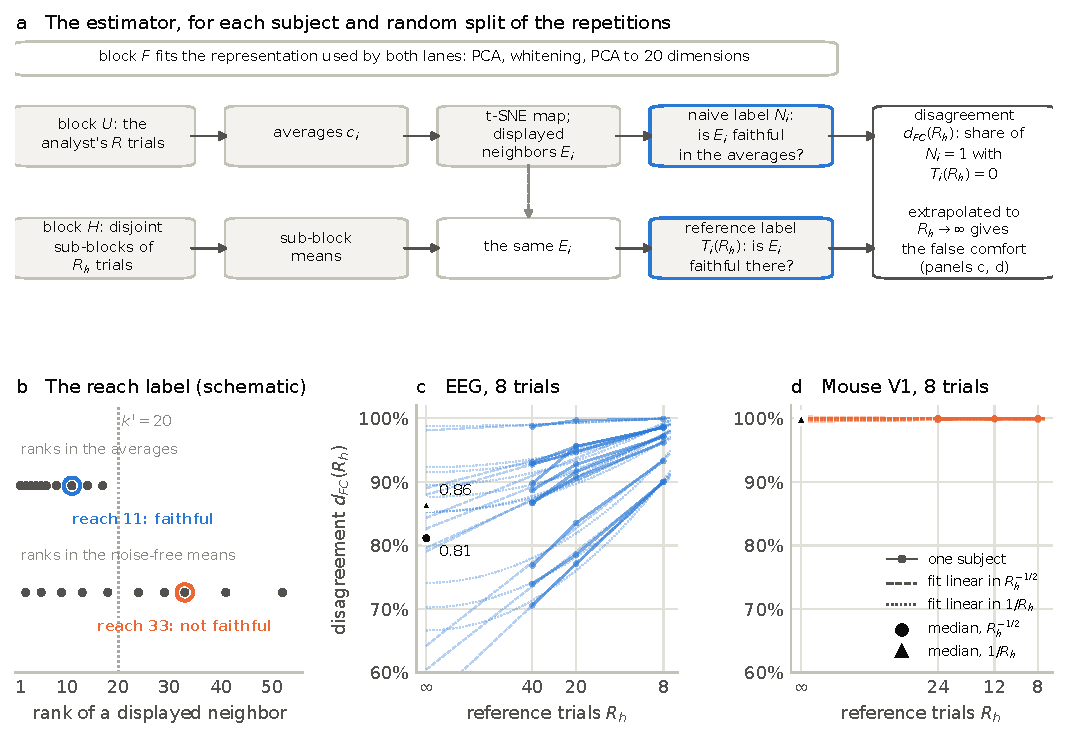
\includegraphics[width=\linewidth]{figures/fig1_method.pdf}
\caption{The estimator. (a)~For each subject and random split, block $F$ fits the
representation, the analyst's $R$ trials from block $U$ give the averages, the map and the naive
labels, and each held-out sub-block of block $H$ gives reference labels for the same displayed
neighborhoods. (b)~The reach label, schematically: a displayed neighborhood of 10 points is
faithful if its 8th-smallest neighbor rank is at most $k'=20$. Here it is faithful in the averages
but not in the noise-free means, a case of false comfort. (c,d)~The disagreement $d_{\FC}(R_h)$
between the naive labels at 8 trials and reference labels of $R_h$ held-out trials, one line per
subject, on an axis linear in $R_h^{-1/2}$. Dashed and dotted lines are the two extrapolants,
linear in $R_h^{-1/2}$ and in $1/R_h$. Their intercepts at $R_h\to\infty$ estimate the false comfort;
black markers are the medians over subjects.}
\label{fig:method}
\end{figure}

\subsection{The estimator recovers a known false comfort}\label{sec:res-plasmode}

In the plasmode simulations the estimator recovered the exact false comfort closely: the median
bias of the conservative estimator at 8 trials was \EegBias{} in EEG and \MouseBias{} in mouse
V1, far inside the pre-specified guard of $\pm0.05$, which therefore never applied
(Supplementary Table~S4). For the common checks of Section~\ref{sec:checks}, the bias ranged from
\ChkBiasMin{} to \ChkBiasMax{} wherever enough neighborhoods passed to check it
(Section~\ref{sec:res-checks}).

\subsection{Most neighborhoods that pass the plug-in check are not faithful}\label{sec:res-main}

\begin{table}[!htb]
\centering\small
\begin{tabular}{llrrrrrr}
\toprule
 & & & Called & Truly & Mislabel & False & Bound \\
Data & Map & Trials & faithful & faithful & rate & comfort & $L$ \\
\midrule
Human EEG & t-SNE & 8 & 18.8 & 4.6--6.6 & 16.9--17.2 & 81--86 & 64 \\
Human EEG & t-SNE & 16 & 26.1 & 9.7--13.8 & 20.8--21.9 & 65--75 & 46 \\
Human EEG & t-SNE & 32 & 32.5 & 16.3--23.3 & 21.0--24.3 & 48--64 & 23 \\
\addlinespace
Human EEG & cv-MDS & 8 & 2.0 & 2.5--3.5 & 3.3--3.9 & 62--72 & 55 \\
Human EEG & cv-MDS & 16 & 5.8 & 4.8--6.6 & 6.4--6.7 & 60--71 & 45 \\
Human EEG & cv-MDS & 32 & 9.5 & 6.3--8.7 & 7.6--8.1 & 44--60 & 38 \\
\addlinespace
Mouse V1 & t-SNE & 8 & 16.1 & 0.0 & 16.1 & 100.0 & 99.7 \\
Mouse V1 & t-SNE & 16 & 17.2 & 0.2 & 17.2 & 99.4--99.6 & 97.7 \\
\addlinespace
Mouse V1 & cv-MDS & 8 & 0.9 & 0.0 & 1.0 & 100.0 & 100.0 \\
Mouse V1 & cv-MDS & 16 & 2.2 & 0.1 & 2.3--2.4 & 100.0 & 98.8 \\
\bottomrule
\end{tabular}

\caption{Neighborhood labels at $k=10$, $\varepsilon=0.2$, $k'=20$, in percent. \emph{Called
faithful}: share of points whose displayed neighborhood passes the plug-in check. \emph{Truly
faithful}: share faithful to the noise-free responses. \emph{False comfort}: share of the passing
neighborhoods that are not faithful. Ranges span the two extrapolants' medians over subjects. $L$
is the conservative lower bound of false comfort on which the claims were judged.}
\label{tab:primary}
\end{table}

\begin{figure}[!htb]
\centering
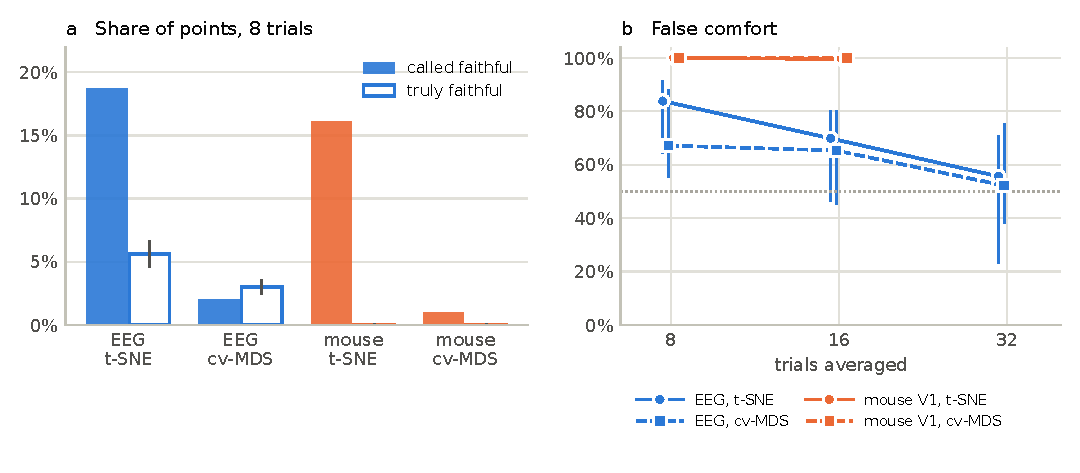
\includegraphics[width=\linewidth]{figures/fig2_false_comfort.pdf}
\caption{(a)~With 8 trials averaged, the plug-in check calls far more neighborhoods faithful than
are faithful in truth; whiskers span the two extrapolants. (b)~False comfort against the number
of trials averaged. Points are the midpoint of the two extrapolants' medians over subjects; bars
run from the conservative bound $L$ to the upper end of the wider 95\% interval. The dotted line
is the 50\% threshold of claims C1 and C1-RSA.}
\label{fig:fc}
\end{figure}

In EEG with 8 trials (Table~\ref{tab:primary}, Figure~\ref{fig:fc}), the plug-in check called
\EegNFeight\% of the t-SNE neighborhoods faithful, while \EegTFeight\% were faithful in truth.
Hence \EegFCeight\% of the passing neighborhoods were not faithful (bound \EegLeight\%), and C1
is supported. More trials helped slowly: false comfort was \EegFCsixteen\% at 16 trials (bound
\EegLsixteen\%) and \EegFCthirtytwo\% at 32 trials, where the bound of \EegLthirtytwo\% falls short
of C2's 25\%, so C2 is not supported. The mislabel rate stayed above 10\% at every budget, with
bounds of \EegQL, supporting C3.

In mouse V1, essentially no displayed neighborhood was faithful in truth: none at 8 trials and
0.2\% at 16. Yet the check called \MouseNFeight\% of them faithful, so the false comfort was
\MouseFCeight\% (bound \MouseLeight\% at 8 trials and \MouseLsixteen\% at 16). C1 and C3 are
supported, the latter with bounds of \MouseQL.

\subsection{Cross-validated distances make the check stricter, not accurate}\label{sec:res-rsa}

Maps of cross-validated distances did not remove false comfort. They made faithful calls rare:
\EegRsaNFeight\% of points in EEG and \MouseRsaNFeight\% in mouse V1 at 8 trials. But most of
those calls were wrong: \EegRsaFCeight\% in EEG (bound \EegRsaLeight\%) and \MouseRsaFCeight\% in
mouse V1 (bound \MouseRsaLeight\%). C1-RSA is supported in both datasets.

\subsection{The result holds across pre-specified variations}\label{sec:res-rob}

\begin{figure}[!htb]
\centering
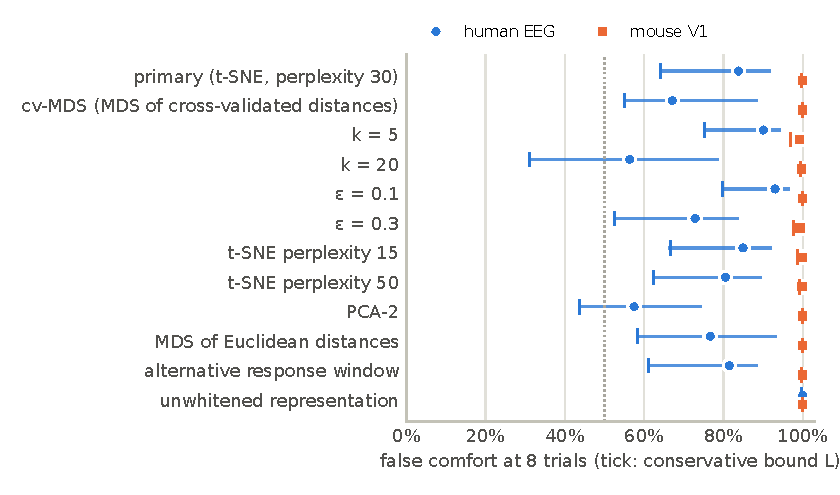
\includegraphics[width=0.8\linewidth]{figures/fig3_robustness.pdf}
\caption{False comfort at 8 trials in the 12 pre-specified variations. Markers are the midpoint of
the two extrapolants; the tick is the conservative bound $L$, which C1 requires to exceed 50\%
(dotted). In EEG it does so in \EegCells{} of 12 variations, in mouse V1 in all 12.}
\label{fig:rob}
\end{figure}

Across variations (Figure~\ref{fig:rob}; Supplementary Tables~S1 and~S2), C1 held in \EegCells{}
of 12 in EEG and therefore counts as general. It failed only on its bound, for $k=20$ (estimate
\EegKtwentyFC\%, bound \EegKtwentyL\%) and for PCA-2 maps (\EegPcaFC\%, bound \EegPcaL\%). In
mouse V1 it held in all 12, and the truly faithful share never exceeded \MouseTFmax\%. Without
whitening, the check called \MouseUnwhitenedNF\% of the mouse neighborhoods faithful and none
were; in EEG, false comfort without whitening was \EegUnwhitenedFC\% at 8 trials. Per-subject
estimates are in Supplementary Table~S3.

\subsection{Common checks do not remove the false comfort}\label{sec:res-checks}

\begin{table}[!htb]
\centering\small
\begin{tabular}{lrrrrrl}
\toprule
 & & False & Bounds & Plug-in false & With & \\
Check & Passes & comfort & $L$, $U$ & comfort flagged & plug-in & Classification \\
\midrule
\multicolumn{7}{l}{\textit{Human EEG}} \\
\quad Plug-in & 18.8 & 81--86 & 64, 92 & -- & -- & -- \\
\quad Trustworthiness & 19.0 & 79--85 & 64, 91 & 27--28 & 77--84 & leaves \\
\quad scDEED & 32.5 & 86--90 & 76, 94 & 39--40 & 77--83 & leaves \\
\quad Cross-validated & 7.9 & 73--81 & 59, 86 & 72--74 & 69--78 & leaves \\
\quad Seed recurrence & 34.6 & 87--91 & 77, 94 & 37--39 & 78--84 & leaves \\
\quad Bootstrap recurrence & 0.0 & n.e. & n.e., n.e. & 100 & n.e. & not evaluable \\
\quad Split-half recurrence & 1.2 & 47--62 & 38, 72 & 97--98 & 36--57 & undetermined \\
\addlinespace
\multicolumn{7}{l}{\textit{Mouse V1}} \\
\quad Plug-in & 16.1 & 100.0 & 99.7, 100.0 & -- & -- & -- \\
\quad Trustworthiness & 16.3 & 100.0 & 99.8, 100.0 & 20 & 100.0 & leaves \\
\quad scDEED & 8.8 & 100.0 & 99.7, 100.0 & 68 & 100.0 & leaves \\
\quad Cross-validated & 2.3 & 100.0 & 97.9, 100.4 & 93 & 100.0 & leaves \\
\quad Seed recurrence & 27.2 & 100.0 & 99.8, 100.0 & 41 & 100.0 & leaves \\
\quad Bootstrap recurrence & 0.0 & n.e. & n.e., n.e. & 100 & n.e. & not evaluable \\
\quad Split-half recurrence & 0.0 & n.e. & n.e., n.e. & 100 & n.e. & not evaluable \\
\bottomrule
\end{tabular}

\caption{Common checks against the truth at 8 trials, in percent; medians over 10 subjects.
\emph{Passes}: share of all points whose neighborhood passes the check. \emph{False comfort}: share
of the passes that are not faithful, as the range of the two extrapolants. $L$, $U$: the
conservative bounds. \emph{Plug-in false comfort flagged}: share of the plug-in check's
false-comfort neighborhoods that the check fails. \emph{With plug-in}: the false comfort of the
check applied on top of the plug-in check. \emph{Classification} (pre-specified): the check leaves most
false comfort if $L>50\%$, removes most if $U<50\%$, and is otherwise undetermined; n.e., not
evaluable, because fewer than 5 subjects had a passing neighborhood. Extrapolated values are not
clipped, so a bound can exceed 100\%.}
\label{tab:checks}
\end{table}

\begin{figure}[!htb]
\centering
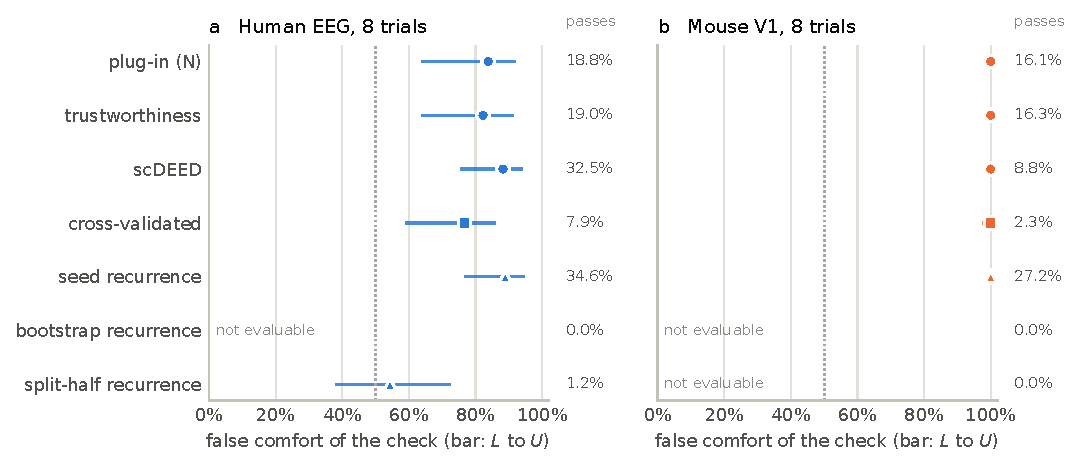
\includegraphics[width=\linewidth]{figures/fig4_checks.pdf}
\caption{Common checks against the truth at 8 trials. Markers are the midpoint of the two
extrapolants' medians over subjects, and bars run from the conservative bound $L$ to $U$; circles
are scores against the averages, the square is cross-validated distances, and triangles are
stability checks. The numbers on the right are the share of all points each check passes. The
dotted line is the 50\% threshold of the pre-specified classification.}
\label{fig:checks}
\end{figure}

The re-created maps reproduced the confirmatory plug-in counts exactly, in all \ChkEegRepRows{}
EEG rows and all \ChkMouseRepRows{} mouse rows, so the six checks were measured on the maps of the
preceding sections. In the plasmode simulations, the conservative estimator's median bias for the
checks' false comfort ranged from \ChkBiasMin{} to \ChkBiasMax{} (Supplementary Table~S7), and the
guard never applied. Bootstrap recurrence passed too few neighborhoods in the simulations for its
estimator to be checked.

Four checks passed as many neighborhoods as the plug-in check or more, and were wrong about as
often (Table~\ref{tab:checks}, Figure~\ref{fig:checks}). In EEG at 8 trials, trustworthiness,
rank-matched to the plug-in check, passed \ChkEegTWPass\% of points with a false comfort of
\ChkEegTWFC\% (bound \ChkEegTWL\%). scDEED's trustworthy label and seed recurrence each passed
about a third of the points (\ChkEegSCDPass\% and \ChkEegSEEDPass\%), with false comfort of
\ChkEegSCDFC\% and \ChkEegSEEDFC\%. About a fifth of all points (\ChkEegExtraSCD\% and
\ChkEegExtraSEED\%) passed them while failing the plug-in check, and those extra passes were mostly not
faithful: stability across seeds and a high score against a permutation null are not faithfulness. Cross-validated distances
passed fewer neighborhoods (\ChkEegCVPass\%) and flagged \ChkEegCVCatch\% of the plug-in check's
false-comfort neighborhoods, but \ChkEegCVFC\% of what they passed was still not faithful (bound
\ChkEegCVL\%). In mouse V1, each of the four was wrong about essentially all it passed (bounds of
at least \ChkMouseMinL\%). By the pre-specified rule, all four leave most false comfort in both
datasets.

The two strict resampling checks passed almost nothing. Bootstrap recurrence, which asks that a
neighborhood recur in 95\% of 50 bootstrap maps, passed essentially no neighborhood at 8 trials in
either dataset, so it was not evaluable. Split-half recurrence passed \ChkEegSHPass\% of the EEG
neighborhoods and essentially none in mouse V1. In EEG it flagged \ChkEegSHCatch\% of the plug-in
check's false comfort, but \ChkEegSHFC\% of the few neighborhoods it passed were still not faithful
(bounds \ChkEegSHL\% and \ChkEegSHU\%), so its classification is undetermined; in mouse V1 it was not
evaluable. None of the six checks removed most false comfort in either dataset.

With more trials, the strict checks began to pass neighborhoods that were more often faithful
(Supplementary Tables~S5 and~S6; these budgets are descriptive, not pre-specified claims). At
32 trials in EEG, split-half recurrence used on top of the plug-in check passed
\ChkEegSHPassNXThirtyTwo\% of points with a false comfort of \ChkEegSHFCNXThirtyTwo\%, against
\EegFCthirtytwo\% for the plug-in check alone. Bootstrap recurrence passed
\ChkEegBOOTPassThirtyTwo\% of points, and its false comfort had an upper bound of
\ChkEegBOOTUThirtyTwo\%, although its estimator could not be validated.


\subsection{Why the check fails: neighbor distances inside the noise (exploratory)}\label{sec:why}

\begin{table}[!htb]
\centering\small
\begin{tabular}{lrr}
\toprule
 & Human EEG & Mouse V1 \\
\midrule
Image pairs with a positive cross-validated distance & 1.000 & 0.937 \\
Split-half reliability of the distance matrix & 0.879 & 0.726 \\
Distance to the 8th nearest image, $d_{(8)}$ & 1.54 & 0.40 \\
Noise between two 16-trial means, $\sigma_{16}$ & 1.68 & 1.65 \\
Ratio $d_{(8)}/\sigma_{16}$ & 0.92 & 0.24 \\
\bottomrule
\end{tabular}

\caption{Exploratory, not pre-specified. One split per subject; medians over subjects. Blocks
$U$ and $H$ of the 20-dimensional representation: 72 repetitions in EEG, 40 in mouse V1, with
distances cross-validated between two halves. $\sigma_{16}$ is the root-mean-square distance
between two independent 16-trial means of the same image.}
\label{tab:snr}
\end{table}

The mouse result is not vacuous (Table~\ref{tab:snr}). Its data contain reliable image-specific
structure: \PosMouse\% of image pairs have a positive cross-validated distance, and the distance
matrix has a split-half reliability of \RelMouse. The trouble is local. The distance from an image
to its 8th nearest neighbor is only \RatioMouse{} times the noise between two 16-trial means, and
for a median of \MouseNonPos{} of the 118 images the cross-validated distance to the 8th nearest image
was not positive even with 40 trials. The
same ratio is \RatioEeg{} in EEG, where a minority of neighborhoods is faithful. In both datasets
the averaged data reproduce the global geometry, while the local ordering that neighborhood labels
depend on stays inside the noise. The map, fitted to the same averages, follows that noise, and a
check computed from the same averages confirms it. We offer the ratio as an account of the
difference between the datasets, not as a tested claim.

\section{Discussion}\label{sec:disc}

% Discussion. discussion_checks.tex and conclusions.tex are written from the comparison's results.

A 2-D map of trial-averaged responses can agree with the averaged data, neighborhood by
neighborhood, and still say little about the responses that the averaging estimates. In two
independent datasets, with claims fixed in advance, most neighborhoods that passed the plug-in
check at 8 trials were not faithful to the noise-free responses: \EegFCeight\% in human EEG and
essentially all in mouse V1. Cross-validated distances made the check stricter but not accurate,
and the result held across the pre-specified variations of the neighborhood definition, the map
and the representation.

\subsection{Implications for practice}

The maps in these data are not meaningless. In both datasets most image pairs were reliably
distinguishable and the distance matrix replicated across independent trials
(Table~\ref{tab:snr}), so the global arrangement of a map, which an RSA noise ceiling would
certify, can be trusted more than its neighborhoods. What fails is the local ordering: the distance
from an image to its 8th nearest neighbor is comparable to, or smaller than, the noise between
two 16-trial means. Five practical consequences follow.
\begin{enumerate}[leftmargin=*]
  \item Neighbor-level readings of maps of few-trial averages (which stimulus sits next to which)
  should be treated as hypotheses, not findings, unless their false comfort has been estimated.
  \item When the design has repetitions to spare, hold some out. With the estimator of
  Section~\ref{sec:est}, a held-out block at two or more sub-block sizes gives the false comfort of
  the analyst's map and of any check the analyst uses, with a conservative bound.
  \item Report that estimate with the map, as one reports a noise ceiling with a model comparison.
  \item Checks computed from the same trials are no substitute. Scores against the averages and
  consistency across t-SNE runs pass many unfaithful neighborhoods. A strict resampling check, such
  as recurrence in maps of both halves of the trials, is the safer of these: at small budgets it
  passes almost nothing, and what it passes is more often faithful than what the permissive checks
  pass.
  \item More trials help slowly. In EEG, false comfort fell from \EegFCeight\% at 8 trials to
  \EegFCthirtytwo\% at 32. Where the ratio of neighbor distance to trial noise is well below one,
  as in mouse V1, no budget in the range studied gives faithful neighborhoods.
\end{enumerate}

\subsection{Comparison with existing methods}

\paragraph{Quality criteria and per-point tools.} Rank-based quality criteria
\citep{venna2001,kaski2003,chen2009,lee2009,venna2010} and per-point tools such as scDEED
\citep{xia2024} and EMBEDR \citep{johnson2022} measure how well a map agrees with the data it was
made from. With trial-averaged data they measure agreement with the averages, and they inherit the
averages' noise. scDEED's permutation null, and EMBEDR's embeddings of randomized data, answer
whether a neighborhood is better preserved than chance, which is a different question from
whether it is faithful to the noise-free responses. In both datasets, per-point trustworthiness and
scDEED's trustworthy label left most false comfort, and scDEED passed more EEG neighborhoods than
the plug-in check without being more often right (Table~\ref{tab:checks}).

\paragraph{Stability.} Recurrence across t-SNE runs, bootstrap resamples (as in DynamicViz;
\citealp{sun2023}) and split halves measures whether a neighborhood is stable, not whether it is
faithful. A neighborhood created by the noise in the averages recurs in every map of those
averages, and a map's systematic distortions recur across seeds and resamples. Seed recurrence
passed a third of the EEG neighborhoods, most of them not faithful. The strict resampling checks
behaved differently: at 8 trials they passed almost nothing, which is itself a useful warning, and
at 32 trials in EEG what they passed was more often faithful. Among the checks we tested, only a
strict resampling check avoided passing many unfaithful neighborhoods, but at 8 trials even
split-half recurrence was wrong about roughly half of the little it passed.

\paragraph{Cross-validated distances and noise ceilings.} RSA's cross-validated distances remove
the positive bias of plug-in distances \citep{walther2016,guggenmos2018}, and noise ceilings bound
how well any model can match a dissimilarity matrix \citep{nili2014,schutt2023}. Neither is
designed to certify single neighborhoods. Cross-validated distances made faithful calls rare, both
as the map's distances (Section~\ref{sec:res-rsa}) and as a check on a t-SNE map, but the calls that
remained were still mostly wrong.

\paragraph{Why checks computed from the same trials cannot see the error.} Under Gaussian trial
noise, the averages carry all the information that the trials hold about the noise-free means; the
residuals add information only about the size of the noise (Supplementary Section~S1.3). Split
halves are the averages plus and minus a noise-only difference, bootstrap resamples are the averages
plus resampled noise, and cross-validated squared distances are the plug-in ones minus a noise-only
term. Every check of Section~\ref{sec:checks} is therefore a function of the averages, the noise
level and randomization. It can be stricter than the plug-in check, but it cannot tell where the
averages themselves are wrong. We recorded this argument, and the prediction that all six checks
would leave most false comfort, in the comparison's protocol before it was run. The prediction held
for the four checks that passed many neighborhoods. The two strict checks did better only by
passing almost nothing: strictness selects the neighborhoods whose margins are large relative to
the noise, and at 8 trials almost none exist. Per-point certificates with family-wise error
control are possible in principle, for instance through simultaneous inference on ranks
\citep{mogstad2024}. In our pilot on THINGS-EEG2, certificates of this kind, built from simultaneous
studentized bounds on pairwise distances, resolved no neighborhood even at 72 trials
(Supplementary Section~S1.5), consistent with Table~\ref{tab:snr}.

\paragraph{Denoised and deeper references.} \citet{lin2024} also judge maps against a denoised
signal, obtained by PCA truncation of the same data, to choose hyperparameters for a whole map. Here
the reference comes from held-out repetitions, it is used at the level of individual neighborhoods,
and false comfort is measured as a function of the number of trials. Downsampling studies compare
neighbor graphs from shallow data with graphs from deeper data \citep{ahlmann2023}, treating the
deeper data as the truth; our extrapolation removes the reference's own noise instead.

\paragraph{What the estimator adds.} The estimator needs held-out repetitions and gives a
dataset-level answer: how much of what a check passes is wrong, with a conservative bound. It does
not certify individual neighborhoods, which the certificates of our pilot could not do at these
signal-to-noise ratios either. It tells an analyst whether reading a map's neighborhoods is
warranted at all, and how false comfort falls as trials are added.


\subsection{Limitations}

Several limitations apply.
\begin{itemize}[leftmargin=*]
  \item \textbf{Scope of the data.} Both datasets are visual responses to static images. Other
  modalities (fMRI, spiking data), other stimulus sets and other response windows may have
  different ratios of neighbor distance to trial noise, and the effect may be weaker where that
  ratio is large.
  \item \textbf{One neighborhood definition.} The definition ($k=10$, $\varepsilon=0.2$,
  $k'=2k$) was varied one factor at a time, not jointly. We tested t-SNE, MDS and PCA maps, but not
  UMAP.
  \item \textbf{The extrapolation assumes a functional form.} We report two extrapolants and judge
  every claim on the more conservative one. The plasmode check found negligible bias, but its truth
  is itself a finite average of held-out trials, so it checks the estimator under the data's noise
  rather than against an exact truth.
  \item \textbf{Shared noise counts as signal.} Noise shared by the analyst's and the reference
  repetitions, such as slow drift within a session, is indistinguishable from signal here. Blocks
  were balanced over sessions (EEG) or over halves of the session (mouse V1) to limit it.
  \item \textbf{Pre-specification.} The EEG confirmation reused the pilot's data with new splits
  and seeds, and pre-specification was by commits to a version-controlled repository rather than
  by an external registry \citep{nosek2018}. The mouse data are the independent test.
  \item \textbf{Representation.} The representation was noise-normalized. Without whitening,
  false comfort in EEG rose to \EegUnwhitenedFC\% at 8 trials; in mouse V1 it was total either way.
  \item \textbf{Sex.} The EEG participants were 8 female and 2 male, and the mice \MouseMale{} male
  and \MouseFemale{} female. With 10 subjects per dataset, we did not analyze sex or gender and
  cannot exclude that either affects the ratio of neighbor distance to trial noise.
  \item \textbf{The comparison of checks} used the primary analysis of each dataset only.
\end{itemize}

\subsection{Conclusions}

At the trial budgets common in systems neuroscience, most neighborhoods that look faithful in 2-D
maps of trial-averaged responses are not faithful to the responses the averaging estimates. Checks
computed from the same trials do not repair this: permissive checks pass many unfaithful
neighborhoods, and strict ones pass almost none. Local neighborhoods in such maps should therefore be
read only against a reference built from held-out repetitions. The estimator presented here
provides one, with a conservative bound, and its code, protocols and results are released with the
paper.



\section*{CRediT authorship contribution statement}
\textbf{Sooyoung Jang:} Conceptualization, Methodology, Validation, Resources, Writing -- review
\& editing, Supervision, Project administration. \todo{confirm the roles}

\section*{Declaration of competing interest}
The author declares no known competing financial interests or personal relationships that could
have appeared to influence the work reported in this paper. \todo{confirm, and complete
the Elsevier declarations tool}

\section*{Funding}
\todo{funding sources and grant numbers, or: This research did not receive any specific grant from
funding agencies in the public, commercial, or not-for-profit sectors.}

\section*{Data availability}
The THINGS-EEG2 preprocessed data are available from the Open Science Framework (project
\texttt{anp5v}) \citep{gifford2022}. The Allen Brain Observatory Visual Coding two-photon data are
available from the Allen Institute's public data store \citep{devries2020}. The code, the
pre-specified protocols with their commit history, the synthetic test logs and all results are
available at \todo{repository URL}.

\section*{Acknowledgements}
We thank the authors of THINGS-EEG2 and the Allen Institute for Brain Science for making their data
openly available.

\section*{Declaration of generative AI and AI-assisted technologies in the manuscript preparation process}
During the preparation of this work the author used Claude (Anthropic; model Claude Opus 5.5) as an
AI research assistant. Under the author's direction, Claude designed and implemented the analyses
and ran them, searched and summarized the literature, and drafted the text, figures and tables.
The author set the research direction, made the decisions reported here, including the choice of
datasets, the journal and every decision to run a pre-specified analysis, and reviewed the
analyses and the text. After using this tool, the author reviewed and edited the content as needed
and takes full responsibility for the content of the published article.

\bibliographystyle{plainnat}
\bibliography{refs}

\end{document}
